\documentclass[review]{elsarticle}

\usepackage{lineno,hyperref}
\usepackage{amsmath}
\usepackage{txfonts}
\usepackage{subcaption}
\usepackage{graphicx}
\modulolinenumbers[5]

\journal{Journal of \LaTeX\ Templates}

%%%%%%%%%%%%%%%%%%%%%%%
%% Elsevier bibliography styles
%%%%%%%%%%%%%%%%%%%%%%%
%% To change the style, put a % in front of the second line of the current style and
%% remove the % from the second line of the style you would like to use.
%%%%%%%%%%%%%%%%%%%%%%%

%% Numbered
%\bibliographystyle{model1-num-names}

%% Numbered without titles
%\bibliographystyle{model1a-num-names}

%% Harvard
%\bibliographystyle{model2-names.bst}\biboptions{authoryear}

%% Vancouver numbered
%\usepackage{numcompress}\bibliographystyle{model3-num-names}

%% Vancouver name/year
%\usepackage{numcompress}\bibliographystyle{model4-names}\biboptions{authoryear}

%% APA style
%\bibliographystyle{model5-names}\biboptions{authoryear}

%% AMA style
%\usepackage{numcompress}\bibliographystyle{model6-num-names}

%% `Elsevier LaTeX' style
\bibliographystyle{model1-num-names}\biboptions{authoryear}
%%%%%%%%%%%%%%%%%%%%%%%

\begin{document}

\begin{frontmatter}

\title{Can linear algebra create perfect knockoffs?\tnoteref{mytitlenote}}
%\tnotetext[mytitlenote]{Fully documented templates are available in the elsarticle package on \href{http://www.ctan.org/tex-archive/macros/latex/contrib/elsarticle}{CTAN}.}

%% Group authors per affiliation:
\author{Christopher Hemmens\fnref{hemmens}}
\author{Stephan Robert\fnref{robert}}
\address{HEIG-VD, Rue de Galilée 15, 1400 Yverdon-les-Bains, Switzerland}
%\fntext[myfootnote]{Since 1880.}

%% or include affiliations in footnotes:
%\author[mymainaddress,mysecondaryaddress]{Elsevier Inc}
%\ead[url]{www.elsevier.com}

%\author[mysecondaryaddress]{Global Customer Service\corref{mycorrespondingauthor}}
%\cortext[mycorrespondingauthor]{Corresponding author}
%\ead{support@elsevier.com}

%\address[mymainaddress]{1600 John F Kennedy Boulevard, Philadelphia}
%\address[mysecondaryaddress]{360 Park Avenue South, New York}

\begin{abstract}
This template helps you to create a properly formatted \LaTeX\ manuscript.
\end{abstract}

\begin{keyword}
Model-X Knockoffs\sep Linear Algebra
\end{keyword}

\end{frontmatter}

%\linenumbers

\section{Introduction}

Ever since its introduction into the literature by \citet{candes2018panning}, Model-X Knockoffs have received a lot of attention. In essence, it is a way of controlling the False Discovery Rate (FDR) by creating statistical doppelgangers of the input features of a machine learning model. By including the original features as well as their knockoffs, one gets a useful tool for identifying features that are being chosen through statistical noise rather than through any real predictive power.

However, research is ongoing as to how to best generate Model-X Knockoffs. \citet{candes2018panning} demonstrates how one can generate them for features that follow a multivariate Normal distribution, but this is rather a narrow scope for the technique. \citet{romano2020deep} uses deep generative models to build a machine for sampling approximate model-X knockoffs for arbitrary and unspecified data distributions. \citet{bates2021metropolized} find that applying the Metropolis-Hastings (MH) algorithm (\citet{metropolis1953equation}, \citet{hastings1970monte}) can produce valid knockoffs, in part due to the time-reversibility of the Monte Carlo Markov Chain method that adapts so well to the core feature of reversibility of the knockoff framework. And \citet{ren2021derandomizing} build on these by introducing a derandomizing step into the selection algorithm such that the knockoffs that are generated are more consistent without compromising statistical power.

We present a method for generating Model-X Knockoffs using linear algebra, which in a perfect world would generate the best possible Knockoffs, but in reality require a frequently impractical amount of computer processing time. We offer a solution that can produce decent Knockoffs using linear algebra that complete in a reasonable amount of time.

\subsection{Model-X Knockoffs Definition}

Definition 3.1 of \citet{candes2018panning} states that the Model-X knockoffs for the family of random variables $X=(X_1,\dots,X_p)$ are a new family of random variables $\tilde{X}=(\tilde{X}_1,\dots,\tilde{X}_p)$ constructed with the following two properties:
\begin{enumerate}
\item for any subset $S\subset\{1,\dots,p\}$, $(X,\tilde{X})_{\text{swap}(S)}\stackrel{d}{=}(X,\tilde{X})$;
\item $\tilde{X}\Perp Y$ $|$ $X$ if there is a response $Y$.
\end{enumerate}

In the above definition, $(X,\tilde{X})_{\text{swap}(S)}$ is obtained from $(X,\tilde{X})$ by swapping the entries $X_j$ and $\tilde{X}_j$ for each $j\in S$; for example, with $p=3$ and $S=\{2,3\}$,

$$(X_1,X_2,X_3,\tilde{X}_1,\tilde{X}_2,\tilde{X}_3)_{\text{swap}(\{2,3\})}\stackrel{d}{=}(X_1,\tilde{X}_2,\tilde{X}_3,\tilde{X}_1,X_2,X_3).$$

\section{Methodology}

Suppose we have a multivariate distribution $$H(x_1,\dots,x_d)=Pr(X_1\le x_1,\dots,X_d\le x_d)$$ where the cumulative distribution function (CDF) of $X_i$ is $F_i:\mathbb{R}\rightarrow [0,1]$. Suppose also that we have a sample of this distribution with $n$ observations. Our goal is to use a linear algebra optimization approach to construct perfect Model-X knockoffs. That is, if the original sample is $\mathcal{X}\equiv(X_1,\dots,X_d)\in \mathbb{R}^{d\times n}$, then we want to find a matrix $\tilde{\mathcal{X}}\equiv(\tilde{X}_1,\dots,\tilde{X}_d)\in \mathbb{R}^{d\times n}$ such that the statistical moments of each feature and the other features are equal to the statistical moments of that feature's knockoff and the other features, as well as between that feature's knockoff and the other features' knockoffs, while minimizing the absolute value of the correlation between each feature and its knockoff.

We focus on equating up to the fourth statistical moment: correlation, coskewness, and cokurtosis. To understand our approach, you have to know that generating knockoffs using linear algebra is disproportionately computationally expensive compared to sampling from a distribution and, as a result, our methodology concentrates on minimizing the amount of work a computer needs to do.

\subsection{Setting Constraints}

We define our (standardized) $(m,k)$-moment between variables $X$ and $Y$ to be 

$$\mu_{m,k}(X,Y) = \frac{\frac{1}{n}\sum_{i=1}^{n}\left((x_i-\mu_{1}(X))^k (y_i-\mu_{1}(Y))^{m-k}\right)}{(\mu_{2}(X))^{k/2}(\mu_{2}(Y))^{(m-k)/2}}$$

where $\mu_{1}(X)=\frac{1}{n}\sum_{i=1}^n x_i$ and $\mu_{2}(X)=\frac{1}{n}\sum_{i=1}^n (x_i-\mu_{1}(X))^2$.

We assume that if two random variables $X_i$ and $\tilde{X}_i$ share the same CDF $F_i$, then if $\mu_{m,k}(X_i,X_j)=\mu_{m,k}(\tilde{X}_i,X_j)$, then $\mu_{m,k}(F_i(X_i),F_j(X_j))=\mu_{m,k}(F_i(\tilde{X}_i),F_j(X_j))$. By acknowledging that we can match the moments of variables using their CDF transformation, we can build our code to only accept uniform random variables, on the basis that all features and knockoffs can be reconstructed into their original distributions using the inverse CDF.

This means our first three constraints on each knockoff are that they fit a uniform distribution with bounds 0 and 1. Specifically,

\begin{enumerate}
	\item The result of a Kolmogorov-Smirnov test with the base distribution being uniform returns a p-value of at least $p_{KS}$\%.
	\item The mean value is between the values $\mu_L$ and $\mu_U$ such that $(\mu_L+\mu_U)/2=0.5$.
	\item The variance is between the values $\sigma_L^2$ and $\sigma_U^2$ such that $(\sigma_L^2+\sigma_U^2)/2=0.0833$.
\end{enumerate}

We also set the bounds to be $\epsilon$ and $1-\epsilon$ where $\epsilon$ is very small and non-zero. We don't set the bounds to be 0 and 1 because most distributions in practical settings have an infinite domain and putting 0 or 1 into the inverse CDF would return infinitely large values.

The next set of constraints are simply that for every value of $i,j=1,\dots,d$ where $i\ne j$, and $2\le m\le 4$ with $1\le k\le (m-1)$, we have

\begin{enumerate}
	\item $\mu_{m,k}(\tilde{X}_i,X_j)=\mu_{m,k}(X_i,X_j)$
	\item $\mu_{m,k}(X_i,\tilde{X}_j)=\mu_{m,k}(X_i,X_j)$
	\item $\mu_{m,k}(\tilde{X}_i,\tilde{X}_j)=\mu_{m,k}(X_i,X_j)$
\end{enumerate}

We are careful not to duplicate any of these constraints, for example, $\mu_{4,1}\left(X_i,\tilde{X}_j\right)$ and $\mu_{4,3}\left(\tilde{X}_j,X_i\right)$ are the same condition, so we only include it once in the optimization process.

\subsection{Optimizing}

Now the constraints are set, we want to optimize the knockoffs such that the correlations between the features and their knockoffs are as close to zero as possible. In many circumstances, it may not be possible to generate knockoffs with zero correlation with their features as the resultant multivariate distribution $(X,\tilde{X})$ still needs to have a covariance matrix that is positive-semidefinite in order to be a valid distribution.

For this reason, we set the minimization value to be the sum of the squared correlations between the features and their knockoffs. Formally,

\begin{equation}
\sum_{i=1}^d \left(\mu_{2,1}\left(X_i,\tilde{X}_i\right)\right)^2
\label{eqn:corr}
\end{equation}

By performing the minimization in this way, we trend all the values to zero while also ensuring that the minimization of absolute correlations far from zero are prioritised over those already close to zero.

\subsection{Initial Guess}

Since this approach is computationally expensive, we want to start as close to a viable solution as possible before running the optimization. That way, if a single iteration of the optimization takes an excessively long time, we can reduce the parameter indicating the maximum number of iterations and be comfortable that we started with something approximating a viable knockoff.

In this paper, we approximate $H(\cdot)$ using the Gaussian copula:

$$H(x_1,\dots,x_d)\approx C(x_1,\dots,x_d)\equiv\Phi\left(\Phi^{-1}(F_1(x_1)),\dots,\Phi^{-1}(F_d(x_d))\right)$$

This approximation allows use to generate an initial guess for the knockoffs that already minimizes (\ref{eqn:corr}) somewhat while matching the covariance constraints using the formula provided in Section 3.1.1 of \citet{candes2018panning}.

All that remains is to set the model's tolerance, maximum iterations, and learning rate.

\section{Speed Test Results}

To test the efficiency of the algorithm, we randomly generate $n$ observations for $d$ independent uniform random variables with bounds 0 and 1. We then shuffle the elements to artificially create non-zero covariance, coskewness, and cokurtosis among the variables. For variable $U_i$,

\begin{itemize}
	\item if mod$(i,4)$ equals 1, we weight smaller observations towards the end of the sample,
	\item if mod$(i,4)$ equals 2, we weight larger observations towards the end of the sample,
	\item if mod$(i,4)$ equals 3, we weight observations close to the mean towards the end of the sample,
	\item if mod$(i,4)$ equals 0, the sample is left unchanged.
\end{itemize}

We run the algorithm using a CPU 11th Gen Intel(R) Core(TM) i7-11700F @ 2.50GHz with 16GB RAM running on Windows 11 Home 64-bit OS. $p_{KS}$ is set to be 10\%, $\mu_L$ and $\mu_U$ are set to cover three standard deviations derived from the means of the features, and $\sigma_L^2$ and $\sigma_U^2$ are set to cover three standard deviations derived from the variances of the features.

In the case of $d=4$ and $n=100$, for example, these bounds are approximately

\begin{itemize}
	\item $\mu_L = 0.442$
	\item $\mu_U = 0.558$
	\item $\sigma^2_L = 0.0517$
	\item $\sigma^2_U = 0.1149$
\end{itemize}

\subsection*{\underline{$d=4$}}

Tables \ref{tbl:summ2} and \ref{tbl:corr2} show how the summary statistics of the knockoffs evolve as more iterations in the knockoff construction process are performed, in addition to the correlation between each feature and its knockoff, which we want to be as close to zero possible.

Because of the way we construct our initial guess, these values are already very close to what we want the final result to be, so they don't vary much as the optimization process continues. The important question is whether the constraints on the moments are fulfilled and, if so, how quickly and how precisely.


\begin{table}
	
$$\begin{array}{r | c | r r | r r | r r}
\text{Knockoff} & \text{Iterations} & \multicolumn{2}{c |}{\text{Mean (0.5)}} & \multicolumn{2}{c |}{\text{Variance (0.083)}} & \multicolumn{2}{c}{\text{Uniform p-value}} \\
 & n= & 100 & 1000 & 100 & 1000 & 100 & 1000 \\
\hline
\tilde{U}_1 & 3 & 0.51 & 0.49 & 0.066 & 0.079 & 33.0\% & 3.4\% \\
 & 10 & 0.52 & 0.49 & 0.079 & 0.079 & 23.3\% & 9.8\% \\
 & 20 & 0.52 & 0.50 & 0.088 & 0.078 & 20.5\% & 7.0\% \\
 \hline
\tilde{U}_2 & 3 & 0.47 & 0.50 & 0.072 & 0.082 & 15.5\% & 16.3\% \\
 & 10 & 0.48 & 0.50 & 0.080 & 0.083 & 33.6\% & 22.8\% \\
 & 20 & 0.48 & 0.50 & 0.073 & 0.083 & 41.5\% & 15.2\% \\
 \hline
\tilde{U}_3 & 3 & 0.55 & 0.51 & 0.086 & 0.081 & 18.9\% & 2.8\% \\
 & 10 & 0.54 & 0.51 & 0.087 & 0.081 & 16.0\% & 3.7\% \\
 & 20 & 0.54 & 0.51 & 0.087 & 0.079 & 44.0\% & 2.8\% \\
 \hline
\tilde{U}_4 & 3 & 0.48 & 0.52 & 0.077 & 0.080 & 67.4\% & 4.0\% \\
 & 10 & 0.48 & 0.52 & 0.078 & 0.081 & 65.0\% & 7.6\% \\
 & 20 & 0.48 & 0.52 & 0.077 & 0.081 & 76.4\% & 5.8\% \\
\end{array}$$
\caption{Summary statistics for the knockoffs when $d=4$}
\label{tbl:summ2}
\end{table}

\begin{table}
	
$$\begin{array}{r | c | c c}
\text{Knockoff} & \text{Iterations} & \multicolumn{2}{c}{\text{Correlation with Feature}} \\
 & n= & 100 & 1000 \\
\hline
\tilde{U}_1 & \text{Initial Guess} & 0.007 & -0.010 \\
 & 3 & 0.002 & 0.012 \\
 & 10 & 0.028 & 0.058 \\
 & 20 & 0.008 & 0.049 \\
\hline
\tilde{U}_2 & \text{Initial Guess} & 0.042 & 0.009 \\
 & 3 & 0.005 & 0.007 \\
 & 10 & 0.048 & 0.015 \\
 & 20 & 0.006 & 0.013 \\
\hline
\tilde{U}_3 & \text{Initial Guess} & -0.076 & -0.011 \\
 & 3 & 0.008 & -0.009 \\
 & 10 & 0.023 & -0.004 \\
 & 20 & 0.001 & 0.003 \\
\hline
\tilde{U}_4 & \text{Initial Guess} & 0.036 & 0.003 \\
 & 3 & 0.028 & 0.005 \\
 & 10 & 0.005 & 0.008 \\
 & 20 & -0.004 & 0.004 \\
\end{array}$$
\caption{Correlation of each feature and its knockoff when $d=4$}
\label{tbl:corr2}
\end{table}

\begin{figure}[h!]
  \centering
   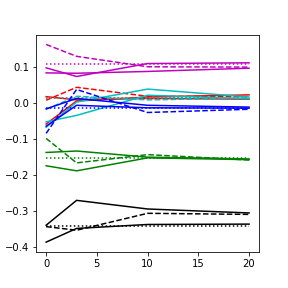
\includegraphics[width=0.33\linewidth]{Graph_2_2_1.png}
   \caption{Evolution of \underline{correlation} constraint adherence over 20 iterations, $d=4$, $n=100$} 
   \label{fig:22corr}
\end{figure}

\begin{figure}[h!]
  \centering
   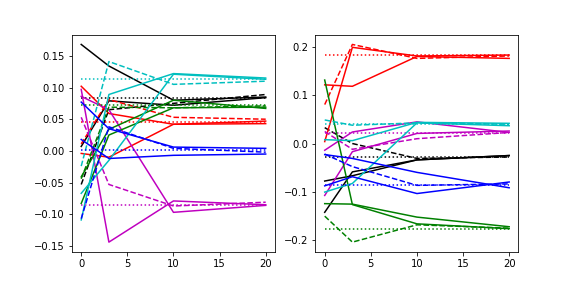
\includegraphics[width=0.67\linewidth]{Graph_2_2_2.png}
   \caption{Evolution of \underline{coskewness} constraint adherence over 20 iterations, $d=4$, $n=100$} 
   \label{fig:22cosk}
\end{figure}

\begin{figure}[h!]
  \centering
   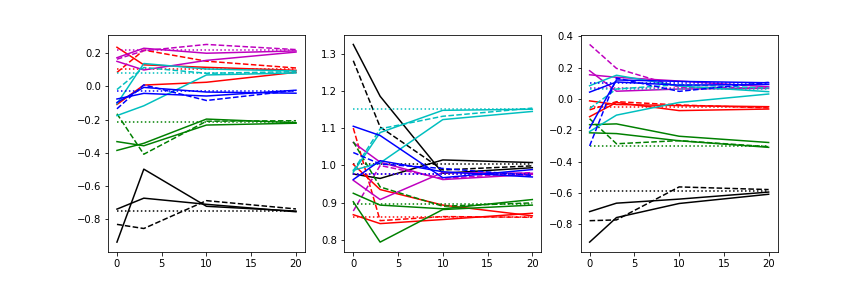
\includegraphics[width=\linewidth]{Graph_2_2_3.png}
   \caption{Evolution of \underline{cokurtosis} constraint adherence over 20 iterations, $d=4$, $n=100$} 
   \label{fig:22coku}
\end{figure}

With four features, we have six relationships whose knockoff moments need to match those of their features. Figures \ref{fig:22corr}, \ref{fig:22cosk}, and \ref{fig:22coku} show the six relationships across the six moments of interest: correlation, left and right coskewness, and left, central, and right cokurtosis, and their evolution as we perform additional iterations in the optimization process. 

Each colour represents a different relationship, for example, black shows the relationship between $U_1$ \& $U_2$, $\tilde{U}_1$ \& $U_2$, $U_1$ \& $\tilde{U}_2$, and $\tilde{U}_1$ \& $\tilde{U}_2$. The dotted line shows the real value of the relationship and therefore the target value of the constraint. The two solid lines show the value of the moment between a feature and a knockoff, while the dashed line shows the value of the moment between the two knockoffs.

We can see that the optimization process is reaching the target moments quickly and precisely with this small dataset so we can be confident that the technique is working and producing close to pseudo-perfect knockoffs.

Figure \ref{fig:coku_conv} shows that if we increase the number of features, we see some degradation in the speed with which the constraints converge. In this context, it's important to note that going from 4 features to 8 increases the number of relationships from 6 to 28. In the current code, all of the cokurtosis constraints, for example, are one constraint. The same is true for coskewness and correlation. This is to make the code as computationally efficient as possible, however, we could make the constraints for left coskewness and right coskewness separate constraints to make them converge sooner. The question is whether the increase in speed of convergence is adequately balanced with the loss of computational efficiency. In Subfigures \ref{fig:coku_22} and \ref{fig:coku_23}, we show all the relationships. In \ref{fig:coku_32} and \ref{fig:coku_33}, we just show the quintiles for the sake of readability.

\begin{figure}[h!]
	\centering
	\begin{subfigure}{0.66\linewidth}
		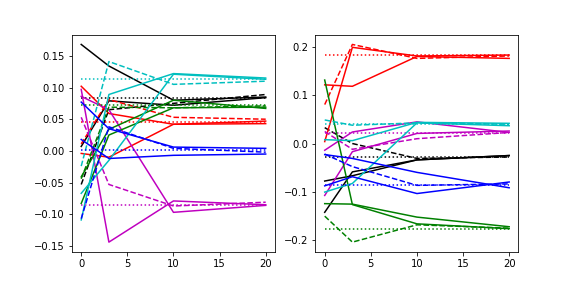
\includegraphics[width=\linewidth]{Graph_2_2_2.png}
		\caption{Coskewness Constraint, $d=4$, $n=100$}
		\label{fig:coku_22}
	\end{subfigure}
	\begin{subfigure}{0.66\linewidth}
		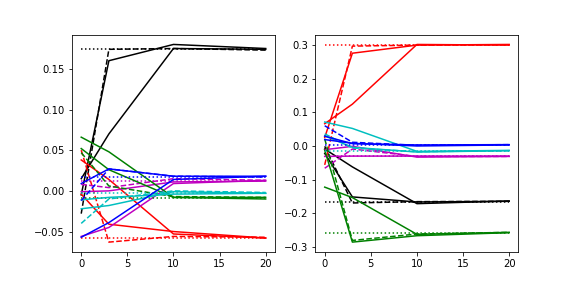
\includegraphics[width=\linewidth]{Graph_2_3_2.png}
		\caption{Coskewness Constraint, $d=4$, $n=1000$}
		\label{fig:coku_23}
	\end{subfigure}
	\begin{subfigure}{0.66\linewidth}
		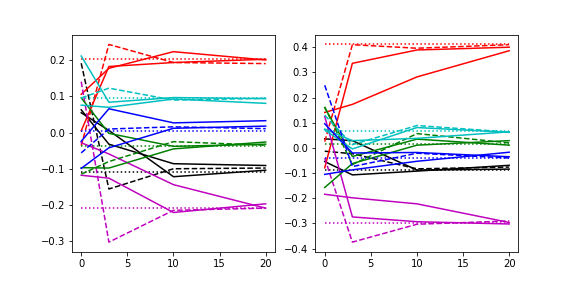
\includegraphics[width=\linewidth]{Graph_3_2_2.png}
		\caption{Coskewness Constraint, $d=8$, $n=100$}
		\label{fig:coku_32}
	\end{subfigure}
	\begin{subfigure}{0.66\linewidth}
		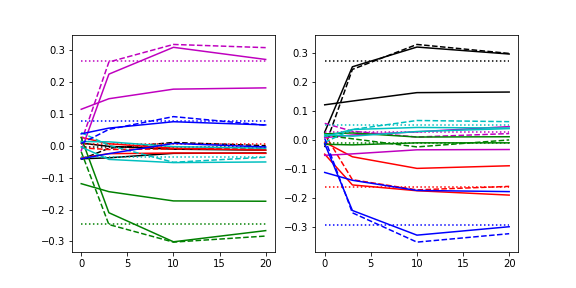
\includegraphics[width=\linewidth]{Graph_3_3_2.png}
		\caption{Coskewness Constraint, $d=8$, $n=1000$}
		\label{fig:coku_33}
	\end{subfigure}
	\caption{Constraint convergence with increasing numbers of features and observations} 
	\label{fig:coku_conv}
\end{figure}

In terms of speed, Table \ref{tbl:time} shows how long each optimization process took. The code is already optimized to scale well with the number of features, $d$. We hope to find additional efficiency savings for the total number of observations.

\begin{table}
	\begin{center}
		
	\begin{tabular}{r r r | c c c}
		\multicolumn{3}{c |}{Total Observations} & \multicolumn{3}{c}{Iterations} \\
		\hline
		$n$ & $d$ & $n\times d$ & 3 & 10 & 20 \\
		\hline
		100 & 4 & 400 & 00:00:09 & 00:00:24 & 00:00:45 \\
		 & 8 & 800 & 00:00:32 & 00:01:32 & 00:02:56 \\
		 \hline
		1000 & 4 & 4000 & 00:08:36 & 00:37:45 & 01:19:17 \\
		 & 8 & 8000 & 01:56:39 & 16:00:54 & 31:53:58 \\
	\end{tabular}
	\end{center}
	\caption{Time taken to complete optimization for a set number of iterations in H:M:S}
	\label{tbl:time}
\end{table}



%The statistical moments for the features and knockoffs are
%
%$$\begin{array}{r | c c c | c c}
%\text{Moment} & \text{Base} & \text{Comparison} & \text{Iterations} & \text{Value w/ Feature} & \text{Value w/ Knockoff} \\
%\hline
%\text{Correlation} & \tilde{U}_1 & U_1 & \text{Real} & 1 & \\
% & & & \text{Initial Guess} & -0.040 & 1  \\
% & & & 3 & -0.009 & 1 \\
% & & & 10 & 0.034 & 1 \\
%\hline
% & \tilde{U}_1 & U_2 & \text{Real} & -0.341 &  \\
% & & & \text{Initial Guess} & -0.265 & -0.310  \\
% & & & 3 & -0.312 & -0.379 \\
% & & & 10 & -0.336 & -0.330 \\
%\hline
% & \tilde{U}_1 & U_3 & \text{Real} & 0.015 &  \\
% & & & \text{Initial Guess} & 0.014 & -0.003  \\
% & & & 3 & 0.027 & -0.021 \\
% & & & 10 & 0.003 & 0.000 \\
%\hline
% & \tilde{U}_1 & U_4 & \text{Real} & 0.108 &  \\
% & & & \text{Initial Guess} & 0.131 & 0.157  \\
% & & & 3 & 0.100 & 0.071 \\
% & & & 10 & 0.094 & 0.116 \\
%\hline
% & \tilde{U}_2 & U_2 & \text{Real} & 1 &  \\
% & & & \text{Initial Guess} & 0.036 & 1  \\
% & & & 3 & 0.030 & 1 \\
% & & & 10 & 0.029 & 1 \\
%\hline
% & \tilde{U}_2 & U_3 & \text{Real} & -0.153 &  \\
% & & & \text{Initial Guess} & -0.316 & -0.215  \\
% & & & 3 & -0.168 & -0.061 \\
% & & & 10 & -0.155 & -0.172 \\
%\hline
% & \tilde{U}_2 & U_4 & \text{Real} & 0.013 &  \\
% & & & \text{Initial Guess} & -0.051 & -0.081  \\
% & & & 3 & 0.008 & 0.031 \\
% & & & 10 & 0.015 & 0.016 \\
%\hline
% & \tilde{U}_3 & U_3 & \text{Real} & 1 &  \\
% & & & \text{Initial Guess} & 0.038 & 1  \\
% & & & 3 & 0.015 & 1 \\
% & & & 10 & 0.035 & 1 \\
%\hline
% & \tilde{U}_3 & U_4 & \text{Real} & -0.014 &  \\
% & & & \text{Initial Guess} & 0.073 & 0.025  \\
% & & & 3 & 0.032 & 0.042 \\
% & & & 10 & 0.013 & -0.007 \\
%\hline
% & \tilde{U}_4 & U_4 & \text{Real} & 1 &  \\
% & & & \text{Initial Guess} & 0.089 & 1  \\
% & & & 3 & 0.052 & 1 \\
% & & & 10 & 0.016 & 1 \\
%\hline
%\end{array}$$


\section{Real Data Results}

To test the effectiveness of this approach on real data, we use daily returns from constituents of the Swiss Market Index (SMI) 




%We start by noting that every parametric distribution has a defined cumulative distribution function (CDF) that can transform each univariate distribution into a uniform distribution with limits 0 and 1. Sklar's Theorem (\citet{sklar1959fonctions}) tells us that any multivariate joint distribution can be represented using a copula. For example, if $H$ is a cumulative distribution function such that
%
%$$H(x_1,\dots,x_d)=Pr(X_1\le x_1,\dots,X_d\le x_d),$$
%
%then there exists a copula $C$ such that
%
%$$H(x_1,\dots,x_d)=C(F_1(x_1),\dots,F_d(x_d))$$
%
%where $F_i(x_i)$ is the marginal cumulative distribution function of random variable $X_i$.
%
%An interesting question that follows from this is whether copulas are a good way of modelling the multivariate probability distribution such that knockoffs are easier to create. A copula, $C:[0,1]^d \rightarrow[0,1]$, describes a joint cumulative distribution function of a d-dimensional random vector on the unit cube $[0,1]^d$ with uniform marginals. (\citet{nelsen2007copula})
%
%Sklar's Theorem (\citet{sklar1959fonctions}) tells us that any multivariate joint distribution can be represented using a copula. For example, if $H$ is a cumulative distribution function such that
%
%$$H(x_1,\dots,x_d)=Pr(X_1\le x_1,\dots,X_d\le x_d),$$
%
%then there exists a copula $C$ such that
%
%$$H(x_1,\dots,x_d)=C(F_1(x_1),\dots,F_d(x_d))$$
%
%where $F_i(x_i)$ is the marginal cumulative distribution function of random variable $X_i$. A consequence of this is that if we can match the co-moments of the uniform variables, then the co-moments of the original variables will also match when the inverse CDFs are applied to the uniform variables.
%
%\citet{candes2018panning} gives us a way of generating Model-X Knockoffs when the features follow a multivariate Normal distribution. Therefore, we can fit our variables to Gaussian copula and use the \citet{candes2018panning} formula to generate an initial guess for our Knockoffs.
%
%Papers that have looked at using copulas to construct knockoffs include \citet{aas2009pair} and \citet{vasquez2023controlling}.
%
%\citet{berti2023new} provide some insight into how copulas can be used to generate knockoffs. If we model our $d$-dimensional cumulative distribution function as a copula,
%
%$$C(F_1(x_1),\dots,F_d(x_d)),$$
%
%then we can replace $F_i(x_i)$ with a 2-copula: $G_i(F_i(x_i),F_i(\tilde{x}_i))$. Here, where $\tilde{x}_i$ represents the knockoff value of $x_i$, you can see that $G_i$ still represents a uniform marginal distribution in the copula, $C$. Since this applies for any 2-copula, and since we want $X_i$ and $\tilde{X}_i$ to be independent, we can choose $G_i$ to be the independence 2-copula: $G_i(u,v)=u\cdot v$.
%
%However, this only generates a valid joint distribution function if the following conditions are satisfied:
%
%In the final part of this introduction, we look at a research field where copulas are frequently used: finance (\citet{embrechts2001modelling}). In the realm of finance, neural networks are often used in the pursuit of index-replicating stock portfolios. The specific technology used is the variational autoencoder, for example, in \citet{heaton2017deep}, in \citet{kim2020index}, and in \citet{zhang2020stock}.
%
%Our goal is to see if this framework can be applied to a branch of research using variational autoencoders 
%
%\section{Methodology -- Linear Algebra}
%
%The first stage in my research involved attempting to generate knockoffs using linear algebra. Ostensibly, the principle of knockoffs means that all the moments between a knockoff and all the other variables should be identical to the moments between the other variables and the original. The only exception is the relationship between the knockoff and the original, which should have as close to no common information as possible.
%
%We can use the result that if any given moment between $Y_1$ and $Y_3$ is the same as the moment between $Y_2$ and $Y_3$, then the moments are also equal for their CDFs. Or, for $1\le k<n$,
%
%$$E\left(Y_1^k \cdot Y_3^{n-k}\right) = E\left(Y_2^k \cdot Y_3^{n-k}\right)$$
%$$\Rightarrow E\left(F(Y_1)^k \cdot G(Y_3)^{n-k}\right) = E\left(F(Y_2)^k \cdot G(Y_3)^{n-k}\right)$$
%
%This way, we can deal entirely with uniform random variables and transform them to the proper random variables later using the CDFs of the marginal distributions. Using linear algebra we can define a set of constraints to generate knockoffs up to a tolerance of $n\ge 2$. These are as follows, $\forall 1\le k< n$, $\forall i$:
%
%$$0<\tilde{U}_i<1$$
%$$E\left(\tilde{U}_i^k\right) \approx \frac{1}{k+1}$$
%$$E(\tilde{U}_i^k U_j^{n-k}) \approx E(\tilde{U}_i^k \tilde{U}_j^{n-k}) \approx E(U_i^k U_j^{n-k}),\, \forall j\ne i$$
%$$E(\tilde{U}_i^k U_i^{n-k}) \approx E(\tilde{U}_i^k) E(U_i^{n-k})\approx\frac{1}{(k+1)(n-k+1)}$$
%
%Theoretically, one can use a linear optimisation algorithm with these constraints to produce perfect knockoffs. There are options available in MATLAB and Python (scipy.optimize).
%
%Unfortunately, even for a small number of features and realisations of those features, the computing power required to generate knockoffs is this manner is too much.

%\section*{References}

\bibliography{knockoff}

\end{document}